\documentclass[11pt,a4paper]{article}
\usepackage[utf8]{inputenc}
\usepackage[T1]{fontenc}
\usepackage{mathptmx}
\usepackage{courier}
\usepackage[margin=0.8in]{geometry}
\usepackage{amsmath,amssymb}
\usepackage{booktabs,tabularx,longtable,array}
\usepackage[shortlabels]{enumitem}
\usepackage{microtype}
\usepackage[dvipsnames]{xcolor}
\usepackage{graphicx,float}
\usepackage[colorlinks=true,linkcolor=NavyBlue,citecolor=NavyBlue,urlcolor=NavyBlue]{hyperref}
\hypersetup{pdftitle={SAFE-Judge: Experimental Supplement},pdfauthor={Ayush Ahuja}}
\usepackage{titlesec}
\usepackage[font=small,labelfont=bf]{caption}
\titleformat{\section}{\large\bfseries}{\thesection}{0.6em}{}
\titleformat{\subsection}{\normalsize\bfseries}{\thesubsection}{0.5em}{}
\titlespacing*{\section}{0pt}{1.3ex}{0.6ex}
\titlespacing*{\subsection}{0pt}{1.0ex}{0.4ex}
\setlist{itemsep=1pt,topsep=3pt,parsep=0pt}
\setlength{\emergencystretch}{2em}
\setlength{\parskip}{2pt}
\setlength{\parindent}{0pt}
\setlength{\textfloatsep}{8pt}
\setlength{\intextsep}{6pt}
\newcolumntype{Y}{>{\raggedright\arraybackslash}X}
\newcolumntype{P}[1]{>{\raggedright\arraybackslash}p{#1}}
\graphicspath{{figures/}}
\renewcommand{\thesection}{\Alph{section}}
\newcommand{\logit}{\operatorname{logit}}
\begin{document}
\begin{center}
{\small COL764: Information Retrieval and Web Search}\\[4pt]
{\Large\bfseries SAFE-Judge: Shared Adaptive Feedback for Escalation\\[2pt]
in Relevance Assessment}\\[6pt]
{\large Final Report: Experimental Supplement}\\[8pt]
\begin{tabular}{rl}
\textbf{Name:} & Ayush Ahuja \\
\textbf{Entry No.:} & 2023CS50911 \\
\end{tabular}
\end{center}
\vspace{-2pt}\hrule\vspace{6pt}
This supplement gives a short account of the additional SAFE-Judge experiments.
The paper presents the method and main results. Full settings, results from each
repeat and records of purchased labels are in \path{artifacts/final/} and the
shared evidence package.

\section{Datasets and Measures}
We developed the method on DL 2019, which has 43 queries and 9,260 pairs.
We then tested the selected settings on DL 2020, with 54 queries and 11,386 pairs.
Grades 2--3 count as relevant in both datasets. The TREC-COVID sample has fifty
topics and 5,000 pairs, with 100 randomly sampled judged pairs per topic.
Grades 1--2 count as relevant. Ten topics are used for development and the other
forty for the main transfer test. Results on all fifty topics include both groups.

The assessor is Qwen3.5-4B, loaded in four-bit form with a 512-token total input
limit. We use the same model weights throughout. Buying a human label means
revealing the official judgment for that pair. Initial checks, calibration
labels and later reviews all count toward the human budget. Selection uses
only labels already bought. DL 2020 and COVID use ten random seeds at each
budget. The cutoff studies use twenty seeds to vary calibration samples and
break ties. Earlier experiments on these public datasets informed development.

Let $A$ be the pairs left for automatic labeling, $D_q$ the pairs for query $q$,
$n_q=|D_q|$, and $N$ the total number of pairs. Let $w_i$ be one when an automatic
label is wrong and zero otherwise. The three error measures use these counts.
\[
 E_Q=\frac1{|Q|}\sum_q\frac{\sum_{i\in A\cap D_q}w_i}{n_q},\qquad
 E_P=\frac{\sum_{i\in A}w_i}{N},\qquad
 R=\frac{\sum_{i\in A}w_i}{|A|}.
\]
$E_Q$ first computes error for each query and then averages across queries.
$E_P$ divides all remaining mistakes by all pairs. Selective error $R$ divides
those mistakes by the automatic pairs. Automatic coverage is $\gamma=|A|/N$,
so $E_P=\gamma R$. Every COVID topic has the same size, giving $E_Q=E_P$.

Macro-F1 summarizes precision and recall across the No/Yes classes. Cohen's
kappa measures agreement after adjusting for chance. Worst-20\% query error
averages the errors of the worst fifth of queries. Worst-class error
$R_{\max}$ is the larger error rate among automatic No and Yes labels.
It is undefined if either class has no automatic labels. $C_+$ is the fraction
of the assessor's original Yes predictions that avoid human review, including
pairs a method later changes to No.

Brier score measures probability error. Ten-bin ECE measures the gap between
predicted probabilities and observed relevance rates. AURC summarizes error
as we accept labels in confidence order, averaging over tied orders.
For review policies, we run each budget separately and release the area over
the measured points separately. Human cost is measured in labels.
For retrieval systems, Kendall's $\tau_b$ and Spearman's $\rho$ compare rankings.
Mean absolute error (MAE) compares nDCG@10 scores, and maximum rank drop measures
the largest downward move. The evaluator also supports MAP for binary labels
and DCG for graded labels.

\textbf{Confidence intervals.} We resample whole queries with replacement,
preserving comparisons between methods. We use 20,000 draws for label error
and 2,000 for ranking and cutoff comparisons. Results are averaged over seeds.
The fitted rules and purchased labels stay fixed during resampling. Reported
95\% intervals therefore describe uncertainty for these fitted policies.
Their interpretation also depends on earlier method selection and the many
comparisons made. Repeating deterministic LARA gives the same result each time.

In the tables, bold marks the best reported mean within a comparable group.
Lower errors and higher F1, kappa, AUC and ranking correlations are better.

\section{Where the Assessor Makes Mistakes}
\begin{center}\small\begin{tabular}{@{}lrrrrrrr@{}}
\toprule
Pool & $N$ & Acc. & F1 & $\kappa$ & Brier & ECE & AURC \\
\midrule
DL 2019 & 9,260 & 79.40 & 0.7368 & 0.4736 & 0.1485 & 0.0688 & 0.1018 \\
DL 2020 & 11,386 & 82.89 & 0.7096 & 0.4235 & 0.1239 & 0.1112 & 0.0710 \\
COVID (40) & 4,000 & 78.08 & 0.7697 & 0.5398 & 0.1551 & 0.0606 & 0.1088 \\
COVID (50) & 5,000 & 78.46 & 0.7736 & 0.5473 & 0.1521 & 0.0558 & 0.1044 \\
\bottomrule
\end{tabular}
\end{center}
In the table, accuracy is a percentage. Other entries range from zero to one.
\begin{figure}[H]\centering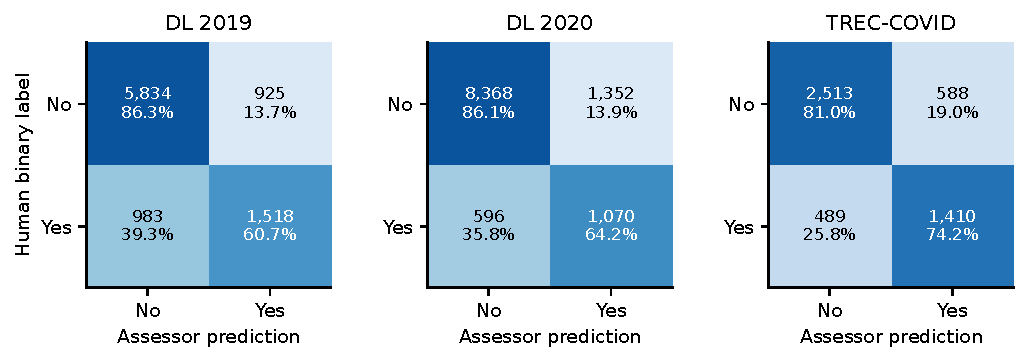
\includegraphics[width=\textwidth]{confusion.pdf}
\caption{Assessor predictions against human labels before review. Rows show
the human class and columns show the prediction. Each cell gives a count and
its percentage within that human class.}
\end{figure}
In the DL 2019 pilot, a confidence cutoff accepted 50.02\% of pairs with 9.78\% selective
error. Confidence worked differently for No and Yes predictions. Some Yes
predictions were highly confident and wrong, which made a single cutoff less
effective. Errors also varied across queries. The worst 20\% of queries held
34.4\% of errors on DL 2019 and 56.7\% on DL 2020, while containing 17.0\% and
27.1\% of pairs. Query size and the share of relevant documents also vary.
These observations led us to test whether feedback from each query improves review.

\begin{figure}[H]\centering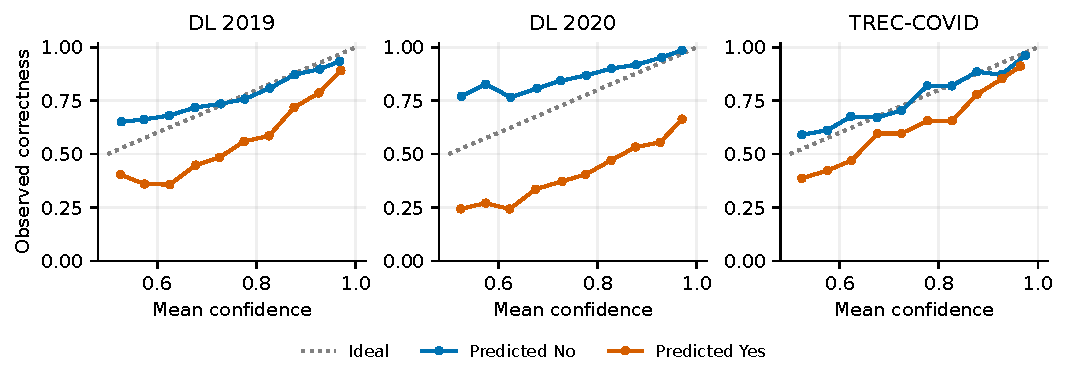
\includegraphics[width=\textwidth]{class_calibration.pdf}
\caption{Model confidence and actual accuracy for No and Yes predictions.
The diagonal shows where confidence matches accuracy. Empty bins are omitted.}
\end{figure}

\section{Review Results on Web and Biomedical Data}
The table compares all four LARA variants, SAFE-Judge, confidence review and
random review at a 50\% human budget. LARA G chooses pairs from the whole pool.
LARA Q gives queries roughly equal review budgets and visits them in turn.
Both update one shared calibrator after each label. Raw and normalized refer
to how probabilities are prepared before LARA runs. SAFE-Judge updates shared
and query-specific error counts, directs the budget using those counts, and
keeps the assessor's labels for unreviewed pairs.

\begin{center}\footnotesize\begin{longtable}{@{}lrrrrrrrr@{}}
\toprule
Pool / method & $E_Q$ & $E_P$ & $R$ & F1 & $\kappa$ & $C_+$ & $R_{\max}$ & Defined \\
\midrule
\endhead
COVID (50) / LARA G/raw & 5.060 & 5.060 & 10.120 & 0.9461 & 0.8921 & 39.94 & 13.16 & 10/10 \\
COVID (50) / LARA G/norm & 5.320 & 5.320 & 10.640 & 0.9436 & 0.8873 & 47.30 & 15.03 & 10/10 \\
COVID (50) / LARA Q/raw & 5.422 & 5.422 & 10.844 & 0.9423 & 0.8846 & 40.65 & 15.26 & 10/10 \\
COVID (50) / LARA Q/norm & 5.728 & 5.728 & 11.456 & 0.9394 & 0.8788 & 47.17 & 16.99 & 10/10 \\
COVID (50) / Random & 10.756 & 10.756 & 21.512 & 0.8863 & 0.7727 & 50.11 & 29.00 & 10/10 \\
COVID (50) / Confidence & 5.084 & 5.084 & 10.168 & 0.9460 & 0.8919 & 43.84 & 13.72 & 10/10 \\
COVID (50) / SAFE-Judge & \textbf{3.950} & \textbf{3.950} & \textbf{7.900} & \textbf{0.9577} & \textbf{0.9154} & 31.31 & 9.11 & 10/10 \\
COVID (40) / LARA G/raw & 5.250 & 5.250 & 10.500 & 0.9439 & 0.8879 & 39.18 & 14.08 & 10/10 \\
COVID (40) / LARA G/norm & 5.425 & 5.425 & 10.850 & 0.9424 & 0.8848 & 46.00 & 15.50 & 10/10 \\
COVID (40) / LARA Q/raw & 5.623 & 5.623 & 11.245 & 0.9401 & 0.8803 & 40.49 & 16.49 & 10/10 \\
COVID (40) / LARA Q/norm & 5.945 & 5.945 & 11.890 & 0.9371 & 0.8742 & 47.20 & 18.21 & 10/10 \\
COVID (40) / Random & 10.950 & 10.950 & 21.900 & 0.8843 & 0.7686 & 49.99 & 30.23 & 10/10 \\
COVID (40) / Confidence & 5.303 & 5.303 & 10.605 & 0.9436 & 0.8871 & 42.90 & 14.88 & 10/10 \\
COVID (40) / SAFE-Judge & \textbf{4.458} & \textbf{4.458} & \textbf{8.915} & \textbf{0.9521} & \textbf{0.9042} & 29.93 & 10.19 & 10/10 \\
DL 2020 / LARA G/raw & 1.086 & 1.379 & 2.758 & 0.9713 & 0.9426 & 0.00 & -- & -- \\
DL 2020 / LARA G/norm & 1.825 & 2.178 & 4.356 & 0.9561 & 0.9122 & 13.34 & 34.06 & 10/10 \\
DL 2020 / LARA Q/raw & 3.612 & 4.995 & 9.989 & 0.9003 & 0.8006 & 22.86 & 52.31 & 10/10 \\
DL 2020 / LARA Q/norm & 4.474 & 6.077 & 12.154 & 0.8852 & 0.7706 & 37.50 & 51.40 & 10/10 \\
DL 2020 / Random & 7.630 & 8.571 & 17.142 & 0.8428 & 0.6863 & 50.16 & 55.65 & 10/10 \\
DL 2020 / Confidence & 2.590 & 3.102 & 6.204 & 0.9394 & 0.8789 & 23.25 & 40.32 & 10/10 \\
DL 2020 / SAFE-Judge & \textbf{0.539} & \textbf{0.667} & \textbf{1.333} & \textbf{0.9864} & \textbf{0.9728} & 0.30 & 1.33 & 8/10 \\
\bottomrule
\end{longtable}
\end{center}
Error and coverage columns are percentages. ``Defined'' counts repeats with
both automatic No and Yes labels. F1 and kappa use the final labels after
human corrections. Each comparison has the same total human-label budget.
Bold compares $E_Q$, $E_P$, $R$, F1 and kappa within each dataset.

At half review, SAFE-Judge leaves 75.9 mistakes on DL 2020, compared with 157
for global raw LARA. The difference in $E_Q$ is $-0.547$ percentage points (pp),
with interval $[-1.119,-0.095]$. On the forty reserved COVID topics, the
difference is $-0.793$ pp, with interval $[-1.748,+0.053]$. This interval
includes zero, so the mean transfer improvement remains uncertain.
Across all fifty COVID topics, errors are 3.950\% and 5.060\%, with difference
interval $[-1.936,-0.364]$ pp. This additional check includes the development
topics and all forty reserved topics. At 90\% review on the reserved topics,
global raw LARA can outperform SAFE-Judge.

\begin{figure}[H]\centering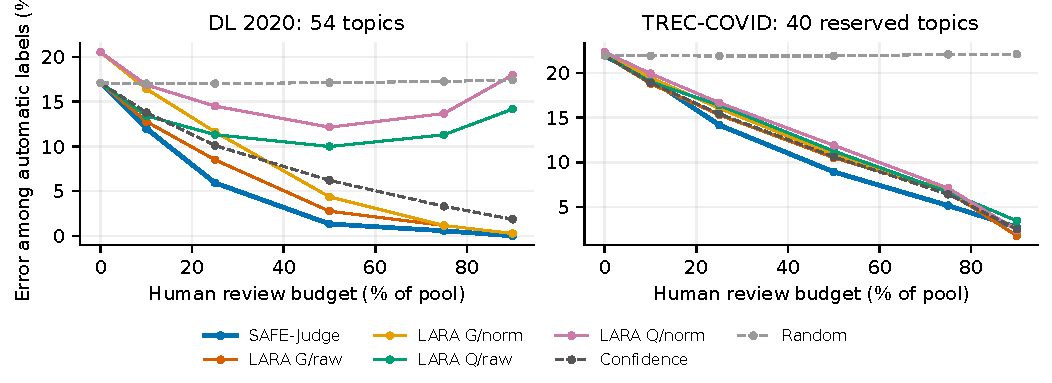
\includegraphics[width=\textwidth]{selective_risk.pdf}
\caption{Error among automatic labels at each total human budget. Each point
comes from a separate review run. Lower is better. The paper plots $E_Q$.}
\end{figure}

\textbf{How much of each class stays automatic.} On DL 2020, SAFE-Judge keeps
only 0.30\% of original Yes predictions automatic. Two of ten runs accept no
Yes labels. Global raw LARA accepts no final Yes labels in all ten runs.
Error for an empty class is undefined. On COVID, SAFE-Judge keeps 29.93\% of
original Yes predictions automatic, with mean worst-class error 10.19\%
compared with LARA's 14.08\%. Class coverage therefore matters when judging
the practical value of a low overall error. Full budget and query-tail results
are in the released tables.

\begin{figure}[H]\centering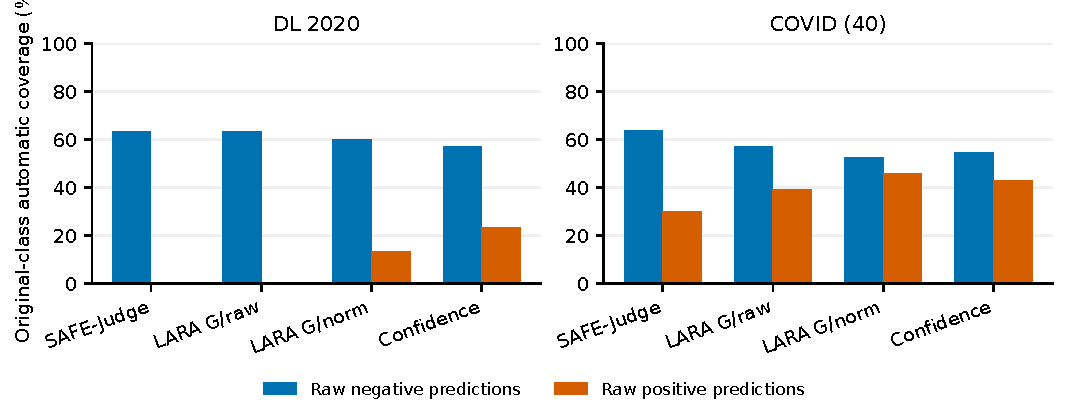
\includegraphics[width=\textwidth]{class_coverage.pdf}
\caption{Original No and Yes predictions left automatic at half review.
Each bar divides automatic pairs by all original predictions of that class.
LARA can change a pair's final label, so these bars describe the original classes.}
\end{figure}

\section{Separate Cutoffs and COVID Calibration}
\textbf{Separate No/Yes cutoffs.} We learn a confidence cutoff for each
predicted class from human labels on separate calibration queries. We choose
cutoffs to reduce the larger class error while keeping at least 5\% of each
original class automatic. Calibration purchases leave fewer labels for direct
test review. The main setting buys 200 labels, with additional tests at 100
and 500. ``Reserved LARA'' is a modified baseline that protects the same 5\%
class coverage. We also report original LARA with the coverage it achieves.
\begin{center}\small\begin{tabular}{@{}llrrrr@{}}
\toprule
Pool & Rule & $R_{\max}$ \% & $C_+$ \% & Coverage \% & Defined \\
\midrule
DL 2020 & LARA G/raw & -- & 0.00 & 50.00 & 0/20 \\
DL 2020 & LARA G/norm & 34.06 & 13.34 & 50.00 & 20/20 \\
DL 2020 & LARA G/raw, 5\% floor & \textbf{23.77} & 5.04 & 50.00 & 20/20 \\
DL 2020 & Confidence & 40.32 & 23.25 & 50.00 & 20/20 \\
DL 2020 & Confidence, paid calibration & 40.33 & 24.69 & 51.76 & 20/20 \\
DL 2020 & Separate class cutoffs & 38.08 & 24.77 & 51.76 & 20/20 \\
COVID (40) & Confidence, paid calibration & 15.51 & 48.36 & 55.00 & 20/20 \\
COVID (40) & Cutoffs, total-error objective & 15.15 & 40.61 & 55.00 & 20/20 \\
COVID (40) & Separate class cutoffs & \textbf{13.86} & 31.28 & 55.00 & 20/20 \\
\bottomrule
\end{tabular}
\end{center}
On DL 2020, separate cutoffs reduce worst-class error from confidence review's
40.32\% to 38.08\%. The difference interval is $[-4.14,-0.17]$ pp.
Normalized global LARA gives 34.06\% and reserved raw LARA gives 23.77\%.
On COVID, separate cutoffs give 13.86\%, compared with confidence review's
14.88\%, raw global LARA's 14.08\% and SAFE-Judge's 10.19\%.
The cutoff comparisons with confidence and LARA have intervals
$[-2.60,1.49]$ and $[-1.49,2.09]$ pp, both including zero.
At equal total cost, the cutoff rule leaves 55\% of test pairs automatic
because 200 labels were spent outside the test pool. Direct review leaves
50\% automatic.

\begin{figure}[H]\centering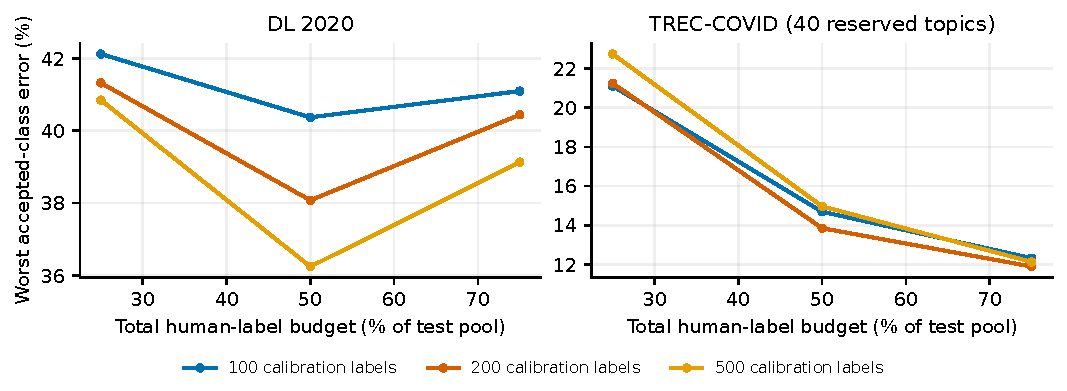
\includegraphics[width=\textwidth]{threshold_calibration_cost.pdf}
\caption{Separate-cutoff results with 100, 200 or 500 calibration labels.
Every calibration purchase counts toward total human cost. Larger calibration
sets leave fewer labels for direct review. Lower worst-class error is better.}
\end{figure}

\begin{figure}[H]\centering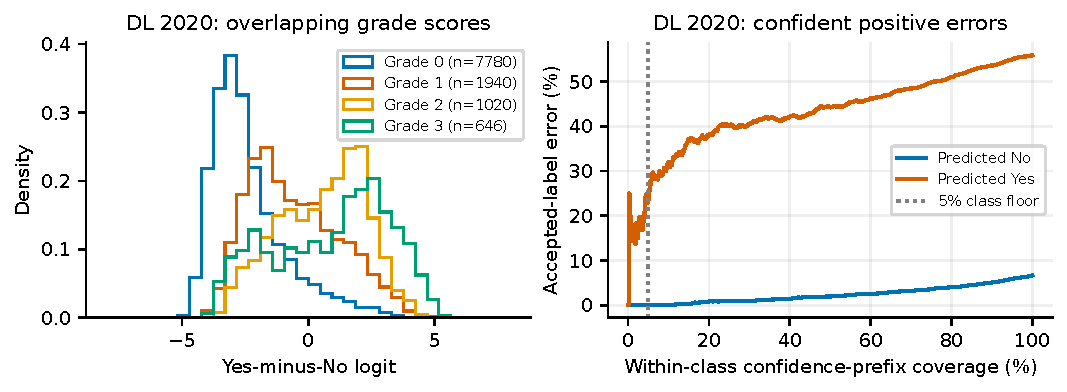
\includegraphics[width=\textwidth]{grade_and_tail_diagnosis.pdf}
\caption{Human relevance grades overlap in the assessor's Yes/No scores.
Highly confident Yes predictions still contain mistakes. These plots use
human grades to study the scores after evaluation.}
\end{figure}
To study the limits of these cutoffs, we also choose the best cutoffs using
all evaluation labels. This idealized check reaches about 23.67\% worst-class
error at the same budget and 5\% class floor. It applies to the tested cutoff
family and tie rules. Confident mistakes, few positive calibration examples
and calibration cost all limit performance. Query feedback can redirect review
toward a difficult query even when its confidence scores resemble other queries.

\textbf{Calibrating probabilities on COVID.} We fit Platt scaling, a logistic
adjustment to the assessor's probabilities, using 200 or 1,000 labels from the
ten development topics. Calibration pairs receive human labels, and further
reviews bring total cost to 2,500. For comparison, raw-score runs buy the same
development labels and use the original probabilities.
\begin{center}\small\begin{tabular}{@{}rllrrr@{}}
\toprule
Cal. labels & Review rule & Scores & $E_P$ \% & $R$ \% & $C_+$ \% \\
\midrule
1000 & LARA G/raw & Platt scaled & 6.100 & 12.200 & 36.39 \\
200 & LARA G/raw & Platt scaled & 5.116 & 10.232 & 33.38 \\
1000 & LARA G/raw & Original & 6.160 & 12.320 & 42.29 \\
200 & LARA G/raw & Original & 5.150 & 10.300 & 40.68 \\
1000 & SAFE-Judge & Platt scaled & 5.690 & 11.380 & 37.04 \\
200 & SAFE-Judge & Platt scaled & 4.542 & 9.084 & 37.98 \\
1000 & SAFE-Judge & Original & \textbf{5.570} & \textbf{11.140} & 33.10 \\
200 & SAFE-Judge & Original & \textbf{4.464} & \textbf{8.928} & 32.52 \\
\bottomrule
\end{tabular}
\end{center}
Bold compares methods with the same number of paid calibration labels.
SAFE-Judge with freely allocated review gives 3.950\% error on the full pool.
Setting aside 200 development labels gives 4.464\%, or 4.542\% with Platt
scaling. Setting aside 1,000 gives 5.570\%, or 5.690\% with scaling.
In these tests, the calibration cost outweighs its benefit. Results use one
fixed development/test split. Reusing calibration labels across later
deployments could reduce the cost per deployment.

\section{Why Query Feedback Helps}
\textbf{Shared feedback and shuffled queries.} We test two changes.
First, use only shared feedback. Second, randomly mix pairs into groups while
keeping group sizes fixed. In these DL 2019 tests, we turn off query-size
weighting for both real and shuffled groups.
\begin{center}\small\begin{tabular}{@{}lr@{}}
\toprule
Grouping / update & $E_Q$ \% \\
\midrule
SAFE-Judge / real queries & \textbf{2.469} \\
Shared-only / real queries & 4.348 \\
SAFE-Judge / shuffled groups & 4.696 \\
Shared-only / shuffled groups & 4.353 \\
\bottomrule
\end{tabular}
\end{center}
The interval for real-query minus shuffled-group SAFE-Judge error is about
$[-4.00,-0.83]$ pp. Shared-only error barely changes when groups are shuffled.
Shuffling also changes the initial checks, so the result measures the full
effect of grouping pairs by query. On DL 2020, shared-only error is 1.270\%
and SAFE-Judge gives 0.539\%. Removing query-size weighting gives 0.540\%.
Query-specific updates account for more of the measured gain in this test.

\textbf{Keeping both classes automatic.} We also test an extension that
chooses reviews to reduce the larger estimated class error while maintaining
a minimum automatic coverage in each class. Its results are reported separately.
\begin{center}\small\begin{tabular}{@{}lrrrr@{}}
\toprule
Allocation & $E_Q$ \% & $R_{\max}$ \% & $C_+$ \% & Defined \\
\midrule
Minimax, query feedback, 5\% floor & \textbf{0.612} & \textbf{10.74} & 5.04 & 10/10 \\
Minimax, query feedback, 20\% floor & 1.697 & 34.19 & 20.02 & 10/10 \\
Query-error objective, 5\% floor & 0.650 & 17.70 & 5.04 & 10/10 \\
SAFE-Judge & 0.539 & 1.33 & 0.30 & 8/10 \\
Minimax, shared-only, 5\% floor & 1.324 & 27.54 & 5.04 & 10/10 \\
\bottomrule
\end{tabular}
\end{center}
Bold compares the three 5\%-floor variants with both classes present in all runs.
The query-feedback extension gives 10.74\% worst-class error with a 5\%
positive-coverage floor. Raising the floor to 20\% raises error to 34.19\%.
Accepting more positive labels automatically increases error in this test.

\textbf{Changing automatic labels and adding extra rules.} DL 2019 query error
is 2.128\% for SAFE-Judge. It becomes 2.559\% with gating, which limits how much
query-specific estimates affect review, and 2.558\% with automatic label correction.
Combining correction, gating and extra exploratory reviews gives 2.879\%.
Shared-only updates give 4.314\%. Correction can turn a correct label into a
mistake. These tests led us to keep the simpler method. A separate sensitivity
study varies the minimum estimated error assigned to highly confident pairs.
That minimum can give different confidence scores the same estimated error.

\textbf{Error predictors and ranking-based review.} We also studied a predictor
that used query information and disagreement with MiniLM. With ten paid initial
labels per query, DL 2019 query error was 2.855\%, compared with raw global
LARA's 4.452\%. Smaller initial samples could perform worse.
Another extension used estimated effects on system rankings when choosing
reviews. On six systems at 10\% review, $\tau_b$ rose from .733 to 1.000 and
score MAE on held-out systems fell from .0495 to .0110. Label error rose from
11.77\% to 13.21\%. With only two held-out systems and fifteen system pairs,
this small study shows how the review objective can affect the result.

\textbf{Learning what counts as relevant.} We also studied learned adjustments
for each query under stricter and looser definitions built from
human grades. Under the usual DL 2020 definition, Brier improved from .1247 to
.0924, while macro-F1 fell from .7093 to .6843. The fraction of relevant pairs
missed rose from 35.82\% to 65.50\%. Under the looser definition, macro-F1 rose
from .7183 to .7520. These outcomes show that better probability estimates can
accompany worse recall. The study varied grade cutoffs. Individual annotator
preferences would require a separate study.

\section{Retrieval System Rankings and Graded Labels}
We compare all 59 official DL 2020 runs using their original top-ten positions
over 54 queries. The main nDCG@10 calculation treats grades 2--3 as relevant.
Its normalization is recomputed from each set of labels. The 1,315 unjudged
positions, covering 1,098 unique pairs, receive zero gain in both calculations.
The results therefore depend on the available judgments.
\begin{center}\small\begin{tabular}{@{}lrrrr@{}}
\toprule
Method & $\tau_b$ & $\rho$ & nDCG MAE & Max drop \\
\midrule
SAFE-Judge & \textbf{0.9882} & \textbf{0.9992} & 0.01128 & \textbf{2.8} \\
LARA G/raw & 0.9871 & 0.9991 & \textbf{0.00299} & 3.0 \\
LARA G/norm & 0.9649 & 0.9968 & 0.02341 & 3.0 \\
LARA Q/raw & 0.9703 & 0.9973 & 0.03105 & 3.0 \\
LARA Q/norm & 0.9681 & 0.9968 & 0.05006 & 3.0 \\
Confidence & 0.9607 & 0.9964 & 0.03832 & 4.0 \\
Random & 0.9409 & 0.9913 & 0.01949 & 5.9 \\
\bottomrule
\end{tabular}
\end{center}
At half review, SAFE-Judge gives $\tau_b=.9882$ and raw global LARA gives .9871.
Their difference interval $[-.0136,.0200]$ includes zero. LARA has lower binary
score MAE, .00299 compared with .01128. Similar rankings can therefore accompany
different score errors. Full automation already gives $\tau_b=.9147$, so the
original .90 target is easy to reach on this pool. Official COVID run analysis
would require a broader judged pool.

\begin{figure}[H]\centering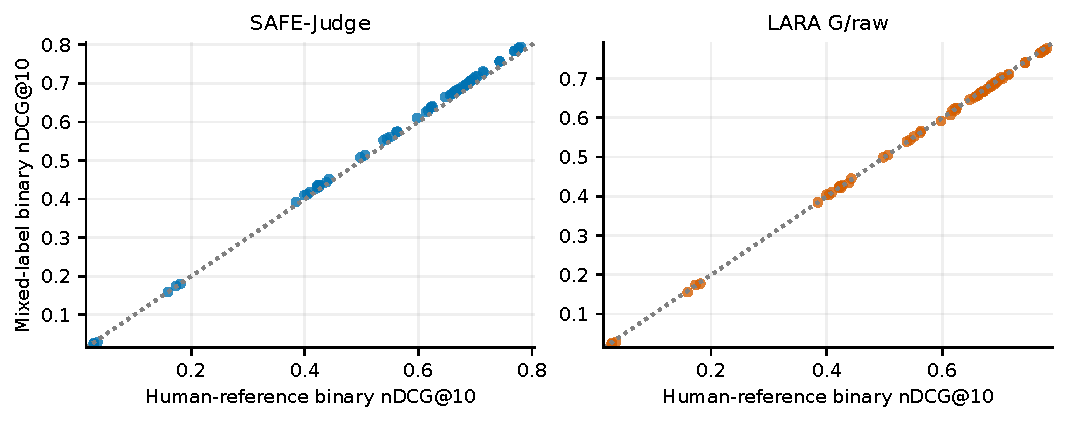
\includegraphics[width=\textwidth]{ranking_fidelity.pdf}
\caption{Mixed-label and human-reference nDCG@10 scores for the 59 official
DL 2020 systems at half review. Each point averages a system's score over
review repeats. The diagonal marks equal scores. Points closer to it indicate
more accurate score estimates.}
\end{figure}

\textbf{Using grades in the ranking calculation.} Reviewed pairs keep their
human grades. Automatic No/Yes predictions are assigned grades 0/2.
With linear gains, SAFE-Judge gives $\tau_b=.9889$ and nDCG MAE .0044,
compared with LARA's .9883 and .0096. These results depend on the chosen 0/2
mapping. Qwen itself supplies binary predictions in this experiment.

\textbf{Predicting grades from paid examples.} We fit linear discriminant
analysis (LDA), quadratic discriminant analysis (QDA) and logistic models using
cached scores and additional features. The 200 source calibration labels count
toward the budget. LDA uses a shared model of score variation across grades.
QDA allows that variation to differ by grade. For binary review, predicted
probabilities of grades 2--3 are added together. Grade scores overlap strongly,
especially for grades 2 and 3. ``Full features'' include the answer-token
probability mass and input length as well as the Yes/No score.
\begin{center}\small\begin{tabular}{@{}lrrrr@{}}
\toprule
Model & Brier & Error AUC & Grade F1 & Grade $\kappa_w$ \\
\midrule
Grade LDA, score & 0.1066 & 0.8505 & 0.3078 & 0.4601 \\
Grade logistic, full features & 0.1043 & 0.8545 & 0.3721 & 0.4768 \\
Grade QDA, full features & 0.1142 & 0.7598 & \textbf{0.3982} & 0.4738 \\
Grade QDA, score & 0.1100 & 0.8136 & 0.3553 & \textbf{0.4810} \\
Binary Platt scaling & \textbf{0.1033} & \textbf{0.8594} & -- & -- \\
Original assessor & 0.1239 & 0.7693 & -- & -- \\
\bottomrule
\end{tabular}
\end{center}
\begin{center}\small\begin{tabular}{@{}lrrr@{}}
\toprule
Rule & $E_Q$ \% & $R$ \% & Coverage \% \\
\midrule
Binary LDA, score & 1.926 & 5.043 & 51.76 \\
Grade LDA, score & \textbf{1.669} & \textbf{4.431} & 51.76 \\
Grade logistic, full features & 1.845 & 4.921 & 51.76 \\
Grade QDA, score & 2.642 & 6.766 & 51.76 \\
Binary Platt scaling & 1.800 & 4.865 & 51.76 \\
\bottomrule
\end{tabular}
\end{center}
Error AUC measures how well a model ranks assessor mistakes, with higher values
better. Grade $\kappa_w$ gives larger penalties to larger grade disagreements.
At half total budget, grade-QDA gives 2.642\% query error and grade-LDA
gives 1.669\%. Binary-LDA gives 1.926\%, raw global LARA gives 1.086\%, and
SAFE-Judge gives 0.539\%. More detailed probability models give higher review
error than SAFE-Judge in these tests. Error limits for each grade and the cost
of supplying graded judgments remain open questions.

\section{Additional Baselines}
\textbf{Classical and neural models on the same test set.} All methods below
use 33 DL 2019 topics, 7,328 pairs, three seeds and 3,664 total human labels.
The lexical model uses BM25, query-term overlap and document length.
MiniLM scores each query and document together. Its temperature-scaling step
adjusts probabilities using 1,932 labels from separate calibration queries,
leaving fewer labels for test review. These comparisons vary both the assessor
and review method. The main LARA comparison uses the same Qwen scores throughout.
\begin{center}\small\begin{tabular}{@{}lrrrrrr@{}}
\toprule
Method & $E_P$ \% & $R$ \% & Coverage \% & Cal. labels & F1 & $\kappa$ \\
\midrule
Lexical active learning & 9.548 & 19.096 & 50.00 & 0 & 0.8632 & 0.7299 \\
MiniLM + temperature & 15.993 & 20.944 & 76.36 & 1932 & 0.8114 & 0.6246 \\
LARA G/norm & 4.326 & 8.652 & 50.00 & 0 & 0.9447 & 0.8895 \\
SAFE-Judge & \textbf{2.543} & \textbf{5.086} & 50.00 & 0 & \textbf{0.9674} & \textbf{0.9348} \\
\bottomrule
\end{tabular}
\end{center}
The lexical model accepts only one predicted class at this budget.
MiniLM scaling improves Brier from .2264 to .1772 and ECE from .2155 to .1528.
Raw macro-F1 stays at .6957. In the pilot's separate Qwen calibration test,
temperature scaling improved Brier and worsened ECE. The measures capture
different aspects of probability quality.

\textbf{Oosterhuis, PPI and CRC.} We use the authors' released Flan-UL2 outputs
and functions to estimate intervals for retrieval scores. Prediction-powered
inference (PPI) combines model predictions with human labels. Conformal risk
control (CRC) uses calibration losses to choose an error-controlled rule.
We check selected calibration sizes. At ten calibration queries, CRC intervals
contain the reference score in .87 of repeats, below the target .95.
At one hundred queries, CRC intervals are narrower in this setup.
Our software environment and data split differ from the original study.
\begin{center}\small\begin{tabular}{@{}lrrrr@{}}
\toprule
Human labels & SAFE-Judge & Best LARA & PPI & CRC midpoint \\
\midrule
220 & 0.7501 & 0.7012 & \textbf{0.1407} & 0.1411 \\
560 & 0.4664 & 0.4848 & \textbf{0.0552} & 0.0757 \\
1130 & 0.0741 & 0.1240 & \textbf{0.0481} & 0.0501 \\
\bottomrule
\end{tabular}
\end{center}
Bold marks the lowest score error at each human-label budget.
The equal-input comparison uses 2,260 top-ten pairs from 226 released TREC-DL
queries. At 1,130 human labels, PPI has lower mean binary DCG error, .0481,
than SAFE-Judge, .0741. SAFE-Judge has lower query-average label error, 3.093\%,
than the best tested LARA mean, 5.177\%. This additional comparison uses an
auxiliary reference pool. Here interval coverage counts how often an interval
contains the reference DCG. We use CRC's interval midpoint when comparing point
estimates. Full interval results and source revisions are released.

\section{Error Checks, Manual Review and Runtime}
\textbf{Spreading calibration labels across queries.} At target error .05,
query CRC uses the correction $(\sum_q L_q+1)/(m+1)$, where $m$ is the number
of calibration queries and $L_q$ is query loss. Fewer than nineteen queries
cannot meet this target even with zero observed errors. Spreading 430 paid
labels across all 43 DL 2019 queries gives 32.37\% automatic coverage and
2.82\% observed query error. Applying this result to new queries or a new
domain requires assumptions about how those queries relate to the calibration data.

\textbf{Auditing the remaining automatic labels.} We draw fresh random labels
from a fixed automatic set and compute conservative error bounds. Every audit
label counts toward human cost. The controller checks for at most 5\%
query-average error, at most 20\% error in each accepted class, and at least
5\% automatic coverage per class. SAFE-Judge passes in only 2/10 DL 2019 runs,
using about 8,610/9,260 human labels on average. On DL 2020, SAFE-Judge, raw
global LARA and confidence review all require full human review in 10/10 runs.
Other audit variants also retain much less automation. In these tests,
certifying the error targets consumes most or all of the saved human effort.

\textbf{Manual review.} We read fifty DL 2019 failures across 31 queries,
including 27 false positives and 23 false negatives. The cases were selected
to study different errors. Category counts describe this selected sample.
\begin{center}\small\begin{tabular}{@{}lr@{}}
\toprule
Category & Count \\
\midrule
Subtle relevance & 9 \\
Keyword distraction & 4 \\
Judgment disagreement & 23 \\
Incomplete answer & 10 \\
Entity mismatch & 3 \\
Domain vocabulary & 1 \\
\bottomrule
\end{tabular}
\end{center}
``Judgment disagreement'' records cases where our reading differs from the
official label. We retain the official labels for evaluation. Partial answers,
subtle relevance and misleading word matches suggest questions for further
study. A study with several reviewers would help assess these explanations.
All fifty case IDs and review notes are released.

\textbf{Runtime and memory.} All three inference runs used one Tesla T4.
\begin{center}\small\begin{tabular}{@{}lrrr@{}}
\toprule
Pool & GPU time (min) & Pairs/s & Truncated \\
\midrule
DL 2019 & 33.12 & 4.66 & 0 \\
DL 2020 & 45.19 & 4.20 & 1 \\
COVID & 32.46 & 2.57 & 1393 \\
\bottomrule
\end{tabular}
\end{center}
COVID inputs were shortened to the token limit in 1,393/5,000 cases.
Longer inputs remain to be tested. DL 2019 used about 3.91 GiB peak allocated
GPU memory and 4.69 GiB reserved memory. Review policies reuse saved scores.
Measured policy times are released for each run. The current implementation
updates priorities for all remaining pairs after each label, taking about
$O(HN)$ work for $H$ purchases and $N$ pairs. Count tables use $O(|Q|)$ storage,
alongside arrays for the pairs. Human reading time and production latency
remain to be measured.

\section{Remaining Work and Shared Files}
The results cover label quality, class coverage, query errors, calibration,
human cost, system rankings, graded-label tests, baseline comparisons, manual
review and runtime. Teacher/QLoRA training, twenty independent topic splits,
repeated-answer consistency tests, prompt variations, longer contexts and a
fresh blind audit remain for future work. Earlier access to public benchmarks
may affect model performance and method selection.

Full settings, source revisions, random seeds and logs are in the shared files.
\path{docs/reproduce_final.md} gives build and replay commands.
\path{docs/experiment_index.md} lists the result files for each study.
The research motivation, interpretation and final experimental decisions are ours.
ChatGPT/Codex assisted with literature review, mathematical formulations, code,
CPU analyses, writing and file preparation. The full disclosure is in
\path{reports/ai_usage_statement.md}. We take responsibility for the claims.
\end{document}
